\documentclass{standalone}
\usepackage{tikz}

\usetikzlibrary{calc,shapes.multipart,shadings}


\begin{document}

\ttfamily
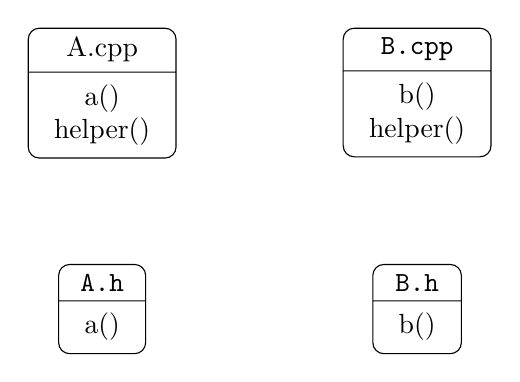
\begin{tikzpicture}[file/.style={rectangle split,rectangle split parts=2,draw,rounded corners=4pt}]
  \node[file,anchor=north] at (0,0) {
    A.cpp
    \nodepart{two}
    \begin{tabular}{c}
      a() \\
      helper()
    \end{tabular}
  };

  \node[file,anchor=north] at (0,-3) {
    \ttfamily A.h
    \nodepart{two}
    \begin{tabular}{c}
      a()
    \end{tabular}
  };

  \node[file,anchor=north] at (4,0) {
    \ttfamily B.cpp
    \nodepart{two}
    \begin{tabular}{c}
      b() \\
      helper()
    \end{tabular}
  };

  \node[file,anchor=north] at (4,-3) {
    \ttfamily B.h
    \nodepart{two}
    \begin{tabular}{c}
      b()
    \end{tabular}
  };
\end{tikzpicture}

\end{document}